\chapter{Parallel Programming and Performance}

	A short introduction to parallel programming and scalability will be given,along with the writers parallel implementation of FSS, a performance and scaling overview and a short comparison with WL.

\section{Parallel Programming}

		A small introduction to two different parallel para-\\digms will be given. As the majority of modern CPUs have at least 4 physical processing cores, CPU code parallelization has become more important then ever to exploit all of the performance provided by modern CPUs. Not only that but as the problem that we are trying to solve becomes more complex or when we want to simulate bigger systems, single core computations may not be able to solve the problem in a reasonable amount of time. This way there is a need for parallelization. GPU computing is also an alternative but, generally, is a more complex approach.

	A program is executed in a process. A process has its own code, data, memory space (stack and a heap), and other specific sets of data. Other processes do not have access to another process data or memory space. A process is executed in only one CPU core. Within a process there is at least one thread, meaning that a process can be single-threaded or multi-threaded. A thread is a sequence of code that is being executed. Each thread has its own stack, and data, however they share the data that is common to the main thread and the heap between them.


		In computer science there are two main paradigms for parallel applications. One based on threads, shared memory parallel programming, and another based on processes, distributed memory parallel programming. 
A shared memory program is executed in multiple threads that coexist in the same memory space. Thus each one has access to the other memory and vice-versa. Therefore communication between concurrent executions of the code within the process is easy. However with multi-threading the code can only be executed in the same computer since it is only run in a single process. Multiple threads running within the same process can reduce parallel performance,. In C/C++, there are many libraries that implement this style of programming, the ones worth mentioning are OpenMP and PThreads. 
On the other hand, a distributed memory concurrent program is executed through various processes each in their own memory space. Communication between processes is harder than thread communication. Multi process communication is more performance taxing since they live in different memory spaces. Excessive communication can lead to performance downfalls, known as communication overhead. This downside, however, comes with better parallel performance and the ability to execute computations in various computing nodes. The default C/C++ library for distributed memory parallel programming is the message passing interface (MPI) having many implementations, such as OpenMPI, MPICH or MVAPICH.


\subsection{Parallel Scalability and Amdahl's Law}

	Consider a certain task that takes a time $T$ to be solved sequentially by one core. Using $N$ workers, ideally, it would only take $T / N$ to complete the task. This is called a speedup on $N$. Ideally, this division of the task assumes that the task can be divided into $N$ pieces of equal complexity, that take the same amount of time to finish. In reality this is not true, the $N$ pieces could have little differences in complexity resulting in some workers having to wait for the other to finish. This is known as load imbalance and induces serialization in the computations.
	
	Let us now construct a model for scalability. Considering the overall problem size is $s + p = 1$, where $s$ is the nonparallelizable part and $p$ is the perfectly parallelizable part.In theory, we would want $s=0$ and $p=1$. In reality, there are many reasons for a nonvanishing serial part. There can be algorithmic limitations meaning that there might be operations that can just not be performed in parallel, bottlenecks in the computer system, such as shared paths to memory between different cores, and communications overhead meaning that in order for workers to inter-communicate there must be some serialization. This last point is often the cause for poor parallel performance. 
		
	The serial wall time can be written as
\begin{equation}
	T_s = s + p,
\end{equation}	
while the wall time of solving the same problem with $N$ workers comes to
\begin{equation}
	T_p = s + \frac{p}{N}.
\end{equation}
This way, application speedup or parallel scalability can be define as the quotient of parallel and serial performance. Serial performance is the serial work done over time
\begin{equation}
	P_s = \frac{s+p}{T_s} = 1,
\end{equation} 
and parallel performance is
\begin{equation}
	P_p = \frac{p+s}{T_p} = \frac{1}{1-p+\frac{p}{N}}.
\end{equation}
The application speedup is now
\begin{equation}
	S = \frac{P_p}{P_s} = \frac{1}{1-p+\frac{p}{N}}.
\end{equation}
This last equation is known as Amdahl's Law, derived by Gene Amdhal in 1967. This limits the speeup when $N \rightarrow \infty$ to $1/(1-p)$. This famous equations tells us how much faster can a program run when using $N$ CPU cores. In Figure \ref{amd_law} the Amdahl's Law speedup is plotted against the number of cores for different values of $p$.
\begin{figure}[h]
	\centering
	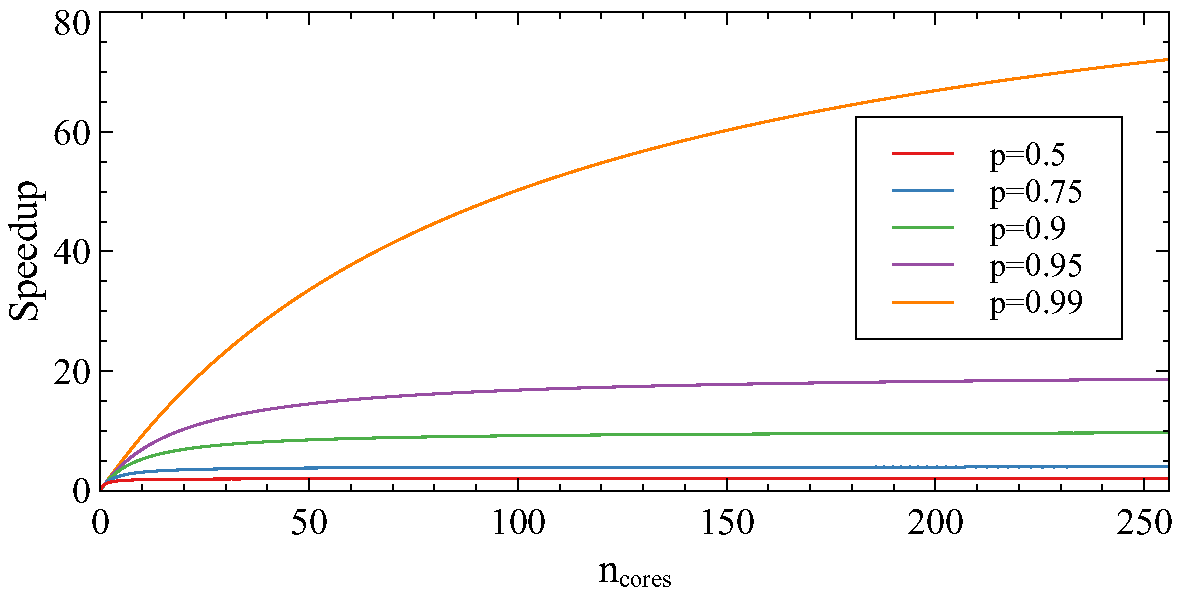
\includegraphics[scale=0.6]{performance/speedup_03.pdf}
	\caption{Speedup from Amdahl's Law as a function of the number of cores for five different values of the parallel portion of the code $p$.}
	\label{amd_law}
\end{figure}

	There are modifications to this law to accommodate system bottlenecks, parallel synchronization and inter-core communications. The most noteworthy is the Hill and Marty's model, which introduces a new way of defining the work and performance. An asymmetric architecture has one manager that does not work and a symmetric architecture has a manager that also does work. The performance of the Hill and Marty's model depends on the type of architecture considered. 
\begin{equation}
		P(N, r) = \twopartdef { \frac{N-r}{r} \sqrt{r} } {\text{symmetric}} {n-r} {\text{assymetric}}
\end{equation}
where $r$ is the size of the sequential core used during the parallel execution.


\section{Implementation}

	Due to the nature of FSS algorithm we can have various independent walkers sampling their own histogram. Each walker performs an independent random walk with access to the whole energy space and constructs a histogram for a magnetization $M_q$. All of the sampled histograms are combined to compute the DoS at $M_{q+1}$. The next iteration is performed using the computed DoS by joining all of the histogram contributions in the last iteration.
This way, in one iteration there is only need for 2 communications. One is the broadcasting of the computed DoS in the last iteration to all of the walkers, the other is the collection of the sampled histograms by all of the walkers. There is a need for one walker to execute all of the serial computations such as the outputting to the terminal and to files, and performing the computations of the DoS at the end of an iteration and broadcasting it to all of the other walkers. Considering this approach, distributed memory parallelism was the better option for a high performant implementation and MPI was used to carry the process to process communications.

	There are two ways of dividing the computations between $n$ walkers. Each performs a random walk with $\text{REP}_{walker} = \text{REP} / n$ giving us the wall time of a single core computation with REP samples per energy divided by the number of walkers or having each walker sample REP configurations per energy giving us the wall time of a single core REP computation.
	
	The MPI implementation starts by assigning each walker a different seed for the RNG, so the results come from different streams of random numbers. This is achieved by multiplying a defined seed by the number assigned to that walker. Then, the first iteration is computed by the manager process and broadcasted to all of the walkers. When all of the walkers have sampled the assigned number of configurations, they send the histogram to the manager and it computes the DoS at the third magnetization finally broadcasts it to the walkers. This is repeated until $q \geqslant q_{max}$. At the end, the manager writes the output files.
 
	Two scenarios of this implementation were explored. One where the manager also performed is own random walk through the energy space, acting like a manager and a walker, and another were the manager only performed the single core operations.Here the advantage is on the side of the first scenario, since there is one more walker and having that walker also performing single core tasks gives an overall better performance than having one idle processes during 95\% of the computation.


\section{Method Performance}

	Now let us discuss the performance of FSS method of both implementations starting by the single core performance and moving on to scaling tests. The following single core benchmarks were performed in a computer equipped with a Ryzen 9 5950X at stock speeds.  
	
	In the following figure, we can observe the wall time and the time spent sampling per energy value as a function of the parameter REP. We can see that the method scales linearly with the parameter REP. 
	
\begin{figure}[ht]
\centering
\subfigure[]{%
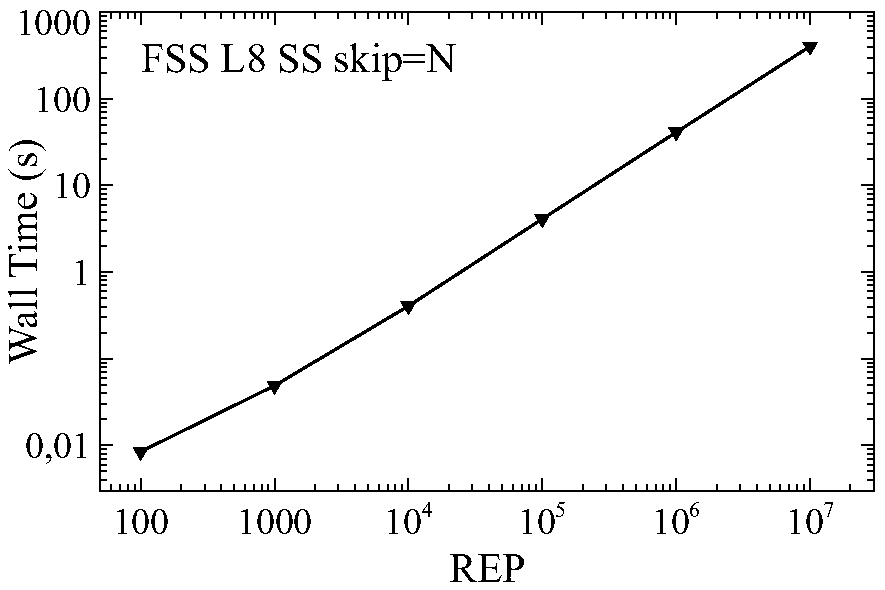
\includegraphics[scale=0.4]{performance/speedup_01.pdf}
\label{L4_wall_time}}
\quad
\quad
\quad
\subfigure[]{%
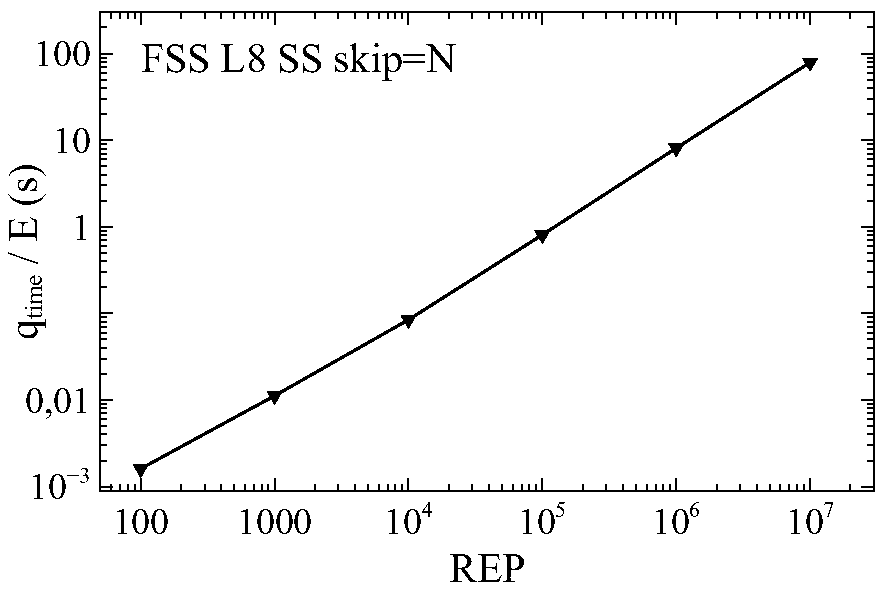
\includegraphics[scale=0.4]{performance/speedup_02.pdf}
\label{L4_wall_time}}	

\caption{(a) LogLog plot of the single core wall time of FSS as a function of the number of samples per each energy point, REP.  (b) LogLog plot of the time spent sampling for each energy value, $q_{time}/E$.These are computations for a system with 16 spins. Data was averaged over 1000 computations to reduce statistical error.}
\end{figure}

Each iteration of the simulation there is an output to the terminal where the $q_{time}/E$ is given. This value is computed by dividing the wall time spent on that iteration by the number of sampled energy points. 
The time spent sampling configurations for each energy value is a very important metric. It can tell us if the computations are stable or the number of samples, REP, must be increased. 
For a stable calculation, this time must remain approximately the same throughout the computation. However, if it is increasing each iteration then usually the value of the parameter REP is insufficient to explore all of the possible energies in the next magnetization. Which causes the estimation of the of the DoS at $M_{q+1}$ to be wrong. In the next iteration the method does not have enough information about the DoS so the time spent sampling will increase. This will propagate until the end of the computations. The obvious solution would be to increase the value of REP, but increasing the skip value is enough, sometimes.

Back to the single core performance. The FSS method scales linearly with the repetitions, so given the wall time of that system with a certain REP value we can easily estimate how much time the computations will take for a another REP value.
When running the algorithm for a new system we can not have a precise estimation for the wall time. However, knowing only the $q_{time}/E$ for the first iterations and assuming that the REP value is sufficient so that this time does not increase, we can estimate the wall time. Assume that the system has $NE$ values of energy and $NM$ values of magnetizations available.The JDoS will have $NE \times NM$ points, but since we only compute half of the JDoS, $( NE \times NM ) / 2$. About $1/3$ to $1/2$ of those points will be different than 0, so the estimation for the wall time comes as 
\begin{equation}\label{estimation}
	\text{Wall Time} \approx (q_{time}/E) \frac{NE \times NM}{2} \times \text{fraction of non-zero points} .
\end{equation}
In Table \ref{wall_time_table} different wall times for single core computations can be seen with the respective estimation through Equation \ref{estimation} for two different fractions of non-zero energy points, $1/3$ and $1/2$. 

\begin{table}[h]
\centering
\caption{Wall Time of some Ising systems with their respective estimations by Equation \ref{estimation} with two different values for the fraction of non-zero energy points.} 
\begin{tabular}{c|c|c|c|c|c|c}
Lattice & $N$   & $NE \times NM$ & $q_{time}/E$ & Wall Time & Estimation $1/3$ & Estimation $1/2$ \\ \hline
SS      & 16  & 289                         & $0.11s $        & $4s$        &$ 5s$                  & $8s$                  \\
SS      & 64  & 4225                        & $0.85s$         & $728s$      & $600s $               & $900s    $ \\
SS      & 256 & 66049                       & $1s$            & $18942s$    & $10898s $             & $16512s  $ \\
SC      & 64  & 6305                        & $1.1s $         & $1148s$     & $1144s$              & $1733s $           \\
FCC     & 256 & 197633                      & $20s$           &$ 871118s$   & $652188s$      & $988165s$            
\end{tabular}
\label{wall_time_table}
\end{table}


\subsection{Parallel Scaling}

	Tests for parallel scalability were performed in the LIP super computer.... 
	

	We can now fit this model to the wall time versus core count data taken from the computations at ...


\begin{figure}[h]
	\centering
	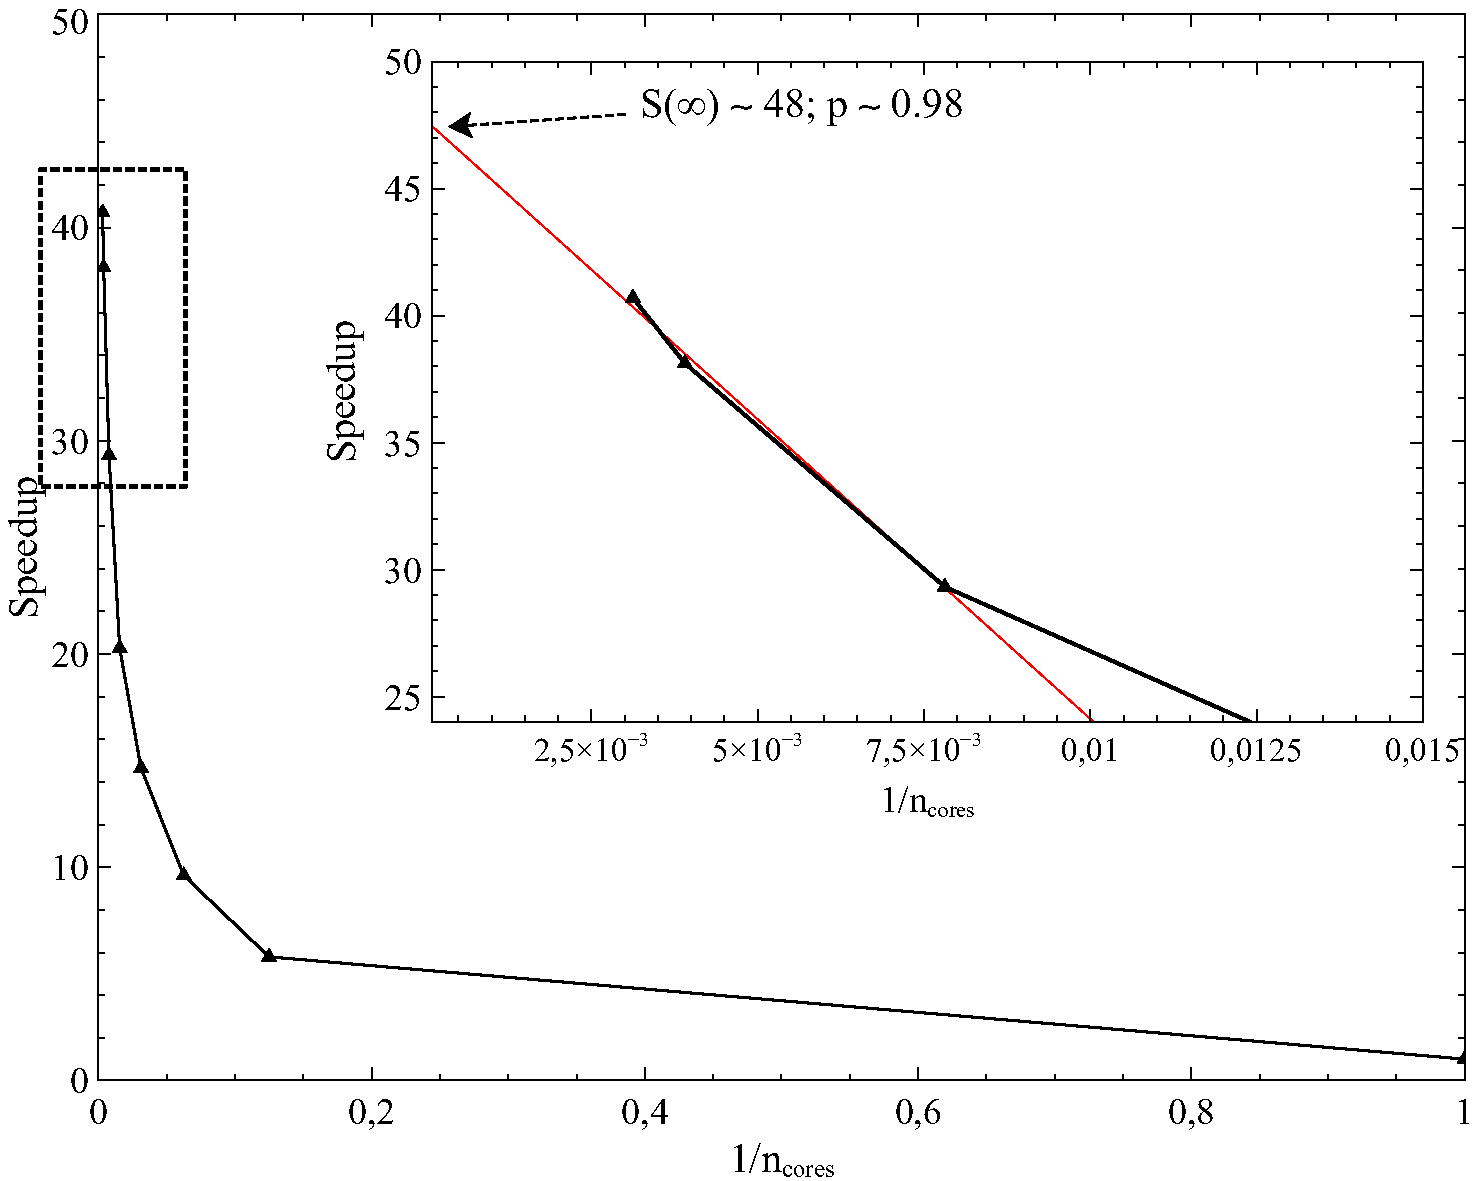
\includegraphics[scale=0.5]{performance/speedup_04.pdf}
	\caption{Extrapolation of the speedup for an infinite number of cores.}
\end{figure}

\begin{figure}[h]
	\centering
	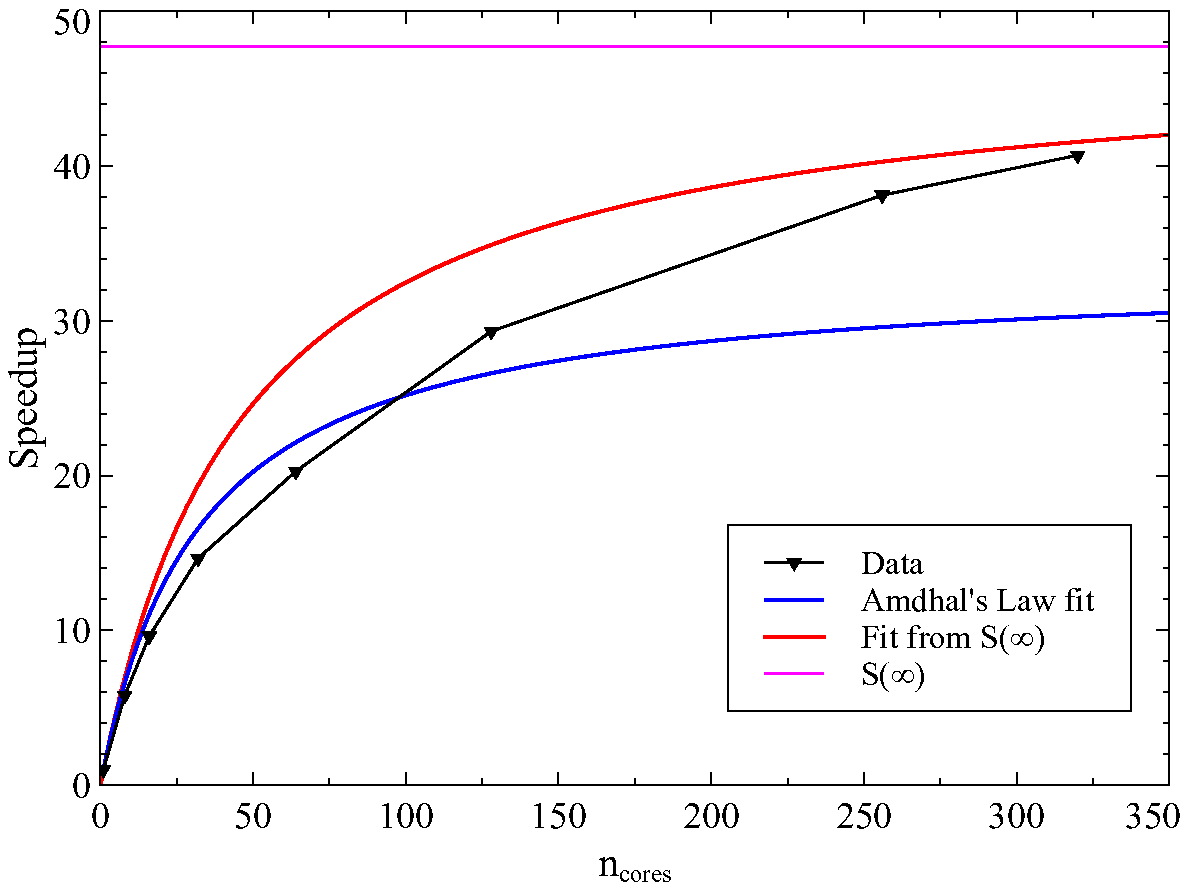
\includegraphics[scale=0.5]{performance/speedup_05.pdf}
	\caption{Amdahl's law fitted for the wall time data.}
\end{figure}


%\section{Comparison with Wang-Landau - Performance}





